\documentclass[twoside]{article}
\setlength{\oddsidemargin}{0.25 in}
\setlength{\evensidemargin}{-0.25 in}
\setlength{\topmargin}{-0.6 in}
\setlength{\textwidth}{6.5 in}
\setlength{\textheight}{8.5 in}
\setlength{\headsep}{0.75 in}
\setlength{\parindent}{0 in}
\setlength{\parskip}{0.1 in}

\usepackage{graphicx}
\usepackage{url}
\usepackage{tikz}

%
% The following commands sets up the lecnum (lecture number)
% counter and make various numbering schemes work relative
% to the lecture number.
%
\newcounter{lecnum}
\renewcommand{\thepage}{\thelecnum-\arabic{page}}
\renewcommand{\thesection}{\thelecnum.\arabic{section}}
\renewcommand{\theequation}{\thelecnum.\arabic{equation}}
\renewcommand{\thefigure}{\thelecnum.\arabic{figure}}
\renewcommand{\thetable}{\thelecnum.\arabic{table}}
\newcommand{\dnl}{\mbox{}\par}

%
% The following macro is used to generate the header.
%
\newcommand{\lecture}[4]{
  \pagestyle{myheadings}
  \thispagestyle{plain}
  \newpage
  \setcounter{lecnum}{#1}
  \setcounter{page}{1}
  \noindent
  \begin{center}
  \framebox{
     \vbox{\vspace{2mm}
   \hbox to 6.28in { {\bf CMPSCI~630~~~Operating Systems
                       \hfill Fall 2014} }
      \vspace{4mm}
      \hbox to 6.28in { {\Large \hfill Lecture #1  \hfill} }
%       \hbox to 6.28in { {\Large \hfill Lecture #1: #2  \hfill} }
      \vspace{2mm}
      \hbox to 6.28in { {\it Lecturer: #3 \hfill Scribe: #4} }
     \vspace{2mm}}
  }
  \end{center}
  \markboth{Lecture #1: #2}{Lecture #1: #2}
  \vspace*{4mm}
}

%
% Convention for citations is authors' initials followed by the year.
% For example, to cite a paper by Leighton and Maggs you would type
% \cite{LM89}, and to cite a paper by Strassen you would type \cite{S69}.
% (To avoid bibliography problems, for now we redefine the \cite command.)
%
\renewcommand{\cite}[1]{[#1]}

% \input{epsf}

%Use this command for a figure; it puts a figure in wherever you want it.
%usage: \fig{NUMBER}{FIGURE-SIZE}{CAPTION}{FILENAME}
\newcommand{\fig}[4]{
           \vspace{0.2 in}
           \setlength{\epsfxsize}{#2}
           \centerline{\epsfbox{#4}}
           \begin{center}
           Figure \thelecnum.#1:~#3
           \end{center}
   }

% Use these for theorems, lemmas, proofs, etc.
\newtheorem{theorem}{Theorem}[lecnum]
\newtheorem{lemma}[theorem]{Lemma}
\newtheorem{proposition}[theorem]{Proposition}
\newtheorem{claim}[theorem]{Claim}
\newtheorem{corollary}[theorem]{Corollary}
\newtheorem{definition}[theorem]{Definition}
\newenvironment{proof}{{\bf Proof:}}{\hfill\rule{2mm}{2mm}}

% Some useful equation alignment commands, borrowed from TeX
\makeatletter
\def\eqalign#1{\,\vcenter{\openup\jot\m@th
 \ialign{\strut\hfil$\displaystyle{##}$&$\displaystyle{{}##}$\hfil
     \crcr#1\crcr}}\,}
\def\eqalignno#1{\displ@y \tabskip\@centering
 \halign to\displaywidth{\hfil$\displaystyle{##}$\tabskip\z@skip
   &$\displaystyle{{}##}$\hfil\tabskip\@centering
   &\llap{$##$}\tabskip\z@skip\crcr
   #1\crcr}}
\def\leqalignno#1{\displ@y \tabskip\@centering
 \halign to\displaywidth{\hfil$\displaystyle{##}$\tabskip\z@skip
   &$\displaystyle{{}##}$\hfil\tabskip\@centering
   &\kern-\displaywidth\rlap{$##$}\tabskip\displaywidth\crcr
   #1\crcr}}
\makeatother

% **** IF YOU WANT TO DEFINE ADDITIONAL MACROS FOR YOURSELF, PUT THEM HERE:



% Some general latex examples and examples making use of the
% macros follow.

\begin{document}

%FILL IN THE RIGHT INFO.
%\lecture{**LECTURE-NUMBER**}{**DATE**}{**LECTURER**}{**SCRIBE**}
\lecture{10}{October 2}{Emery Berger}{Ian Gemp, Patrick Pegus}

\section{Queuing Theory}

\subsection{Little's Law}
%http://tex.stackexchange.com/questions/119597/how-can-i-create-a-queuing-node-using-tikz
\begin{tikzpicture}[>=latex]
% the rectangle with vertical rules
\draw (0,0) -- ++(2cm,0) -- ++(0,-1.5cm) -- ++(-2cm,0);
\foreach \i in {1,...,4}
  \draw (2cm-\i*10pt,0) -- +(0,-1.5cm);

% the circle
\draw (2.75,-0.75cm) circle [radius=0.75cm];

% the arrows and labels
\draw[->] (3.5,-0.75) -- +(20pt,0);
\draw[<-] (0,-0.75) -- +(-20pt,0) node[left] {$\lambda$};
\node at (2.75,-0.75cm) {$W$};
\node[align=center] at (1cm,-2cm) {Queue};
\node[align=center] at (3cm,-2cm) {Servicer};
\end{tikzpicture} \\
$L = \lambda W$ where $L$ is the average queue length, $\lambda$ is the average arrival rate, and $W$ is the average wait time.\\
\\
Requirements/Assumptions:\\
1) Queue can never be empty (i.e. must be ``back-filled'')\\
2) There can't be any crazy feedback processes (i.e. reasonable independence)\\
3) The queue must be in a steady state\\
\\
Little's law is important because of its widespread applicability to a large set of complex queuing problems and its simplicity.\\

\subsection{Latency vs Throughput}
Latency: Waiting Time\\
Throughput/Bandwidth: transactions/sec, queries/sec, etc.\\
- Systems require warm up: Time per byte $\propto$ 1 / bytes transmitted
\begin{enumerate}
\item Old school: Cared about throughput
	\begin{enumerate}
	\item Batch computing: Share a large number of CPUs
		\item Pro: High throughput - schedule tasks so that the all the CPUs are always working
		\item Con: High latency - Might have to wait a long time for your process to initiate due to priority scheduling
	\end{enumerate}
\item New school: Care about latency
	\begin{enumerate}
	\item Facebook focuses on TTI (Time to Interact) metric
	\item 30\% of users close Youtube videos after 1 sec of waiting, 70\% after 3 sec
	\item Interactive computing:
		\begin{enumerate}
		\item 40 to 500 ms latency is acceptable, 24 fps gives us persistence of vision
		\item Try to hide network latency with caching and prefetching
		\item Offload some processes to the client
			\begin{enumerate}
			\item Memoization - memorization of previous function evaluations (from DP)
			\item Buffering
			\item Concurrent local updates with batching (e.g. Google Drive - ``saved'')
			\item Gmail downloads 1.5Mb of javascript
			\end{enumerate}
		\end{enumerate}
	\end{enumerate}
\end{enumerate}

\subsection{MS Outlook}
All mail is stored in a massive .pst file with a single lock (i.e. it is not randomly accessible).  They attempted to use multithreading to simulate concurrency and speed up mail retrieval, but this failed because all of their fetch and send mail requests bottlenecked when accessing the .pst file because of the single lock.  They realized this after creating a queuing network model (QNM) which revealed the basic structure of their queuing network.\\
MS products have been evolving since the 80's and a lot of their code is maintained from previous generations.  Designing from scratch is seldom an option given the size of these projects and maintaining big picture models is very difficult.
\subsection{Why do most software projects not have a performance model?}
\begin{enumerate}
	\item Since the model is not apparent in the code, it must be constructed manually.
	\item The likelihood of a successful project is low. There is no financial gain from developing a model for a project that will probably fail.
	\item Software is built to implement a feature often without concern for performance.
\end{enumerate}

\subsection{Flux}
Allows you to easily extract QNMs from your network by decoupling the software into 4 types: threads, thread-pools, processes, and events.  This could prevent disasters such as the outlook fiasco described above.
\end{document}
